\documentclass[conference]{IEEEtran}

\usepackage{cite}
\usepackage{amsmath,amssymb}
\usepackage{graphicx}
\usepackage{booktabs}
\usepackage{tikz}
\usepackage{xcolor}
\usepackage{hyperref}
\usepackage{pgfplots}
\pgfplotsset{compat=newest}

\hypersetup{
    colorlinks=true,
    linkcolor=blue,
    citecolor=blue,
    urlcolor=blue
}

\begin{document}

\title{Historical Case Study on Ti Silicide (TiSi\textsubscript{2}) \\ Reliability Issues in Legacy CMOS Nodes}

\author{
\IEEEauthorblockN{Shinichi Samizo}
\IEEEauthorblockA{Independent Semiconductor Researcher\\
Project Design Hub, Samizo-AITL\\
\textit{Email:} \href{mailto:shin3t72@gmail.com}{shin3t72@gmail.com}\quad
\textit{GitHub:} \href{https://github.com/Samizo-AITL}{Samizo-AITL}}
}

\maketitle

\begin{abstract}
This paper analyzes a historical failure case related to Ti silicide (TiSi\textsubscript{2}) phase transition instability at the 0.25~µm CMOS node. 
For aTFT-LCD driver ICs requiring $\sim$30~V devices, manufacturers selected the 0.25~µm node because its LOCOS isolation allowed co-integration of existing 30~V modules without redesign. 
In contrast, migrating to 0.18~µm (STI) required a new HV platform. 
Under this context, incomplete C49$\rightarrow$C54 transformation with boron absorption created localized high-resistance spots, directly reducing SRAM yield. 
The case further illustrates how process optimization and empirical feedback cycles became indispensable in semiconductor development under market and cost pressure.
\end{abstract}

\section{Introduction}
Around 2000, the demand for large SRAM and mixed-signal logic in aTFT-LCD drivers surged. 
To ensure reliable 30~V IC functions, many manufacturers adopted the 0.25~µm LOCOS-based node, which was compatible with existing HV device modules. 
In contrast, migrating to 0.18~µm (STI) required a new STI-compatible 30~V device development, posing schedule and ramp risks. 
This decision context exposed vulnerabilities when Ti silicide instabilities degraded yield.

\section{Technical Background}
TiSi\textsubscript{2} was widely adopted for its low resistivity. 
However, the silicide undergoes a phase transition from metastable C49 to stable C54 during rapid thermal annealing (RTA). 
If the transition is incomplete, residual C49 grains act as high-resistance regions. 
Furthermore, boron absorption into TiSi\textsubscript{2} aggravated resistance fluctuation, directly manifesting as random SRAM bit failures.

Additionally, the isolation scheme played a crucial role:
\begin{itemize}
  \item 0.25~µm LOCOS: Mature, thick field oxide, tolerant for HV ($\sim$30~V) integration.
  \item 0.18~µm STI: Shallow trench, better density, but required re-development of HV devices.
\end{itemize}

\section{Node Trade-off: 0.25 µm vs 0.18 µm}
Table~\ref{tab:node} summarizes the trade-offs.  
The 0.25~µm LOCOS node was not simply a cost-driven ``extension,'' but a strategic choice to guarantee HV compatibility with existing aTFT driver requirements.

\begin{table}[!t]
\caption{Comparison of 0.25 µm (LOCOS) and 0.18 µm (STI) CMOS Nodes for aTFT driver ICs}
\label{tab:node}
\centering
\begin{tabular}{@{}lll@{}}
\toprule
 & \textbf{0.25 µm (LOCOS)} & \textbf{0.18 µm (STI)} \\
\midrule
Isolation & LOCOS (thick FOX) & STI (shallow trench) \\
HV integration & Use existing 30V & New 30V platform needed \\
Mask count & $\sim$25 & $\sim$28 \\
Die size / yield & Larger / yield-limited & Smaller / higher density \\
Main risk & TiSi\textsubscript{2} instability & HV redevelopment risk \\
Cost note & Simpler flow & Higher mask/process cost \\
\bottomrule
\end{tabular}
\end{table}

\section{Failure Analysis}
The yield impact was confirmed through SRAM testing.  
Without redundancy, single-bit random defects directly caused device rejection.  
Failure localization pointed to silicide regions at transistor contacts, with boron diffusion assisting local resistivity increase.

% ===== 図をここに配置 =====
\begin{figure}[!t]
  \centering
  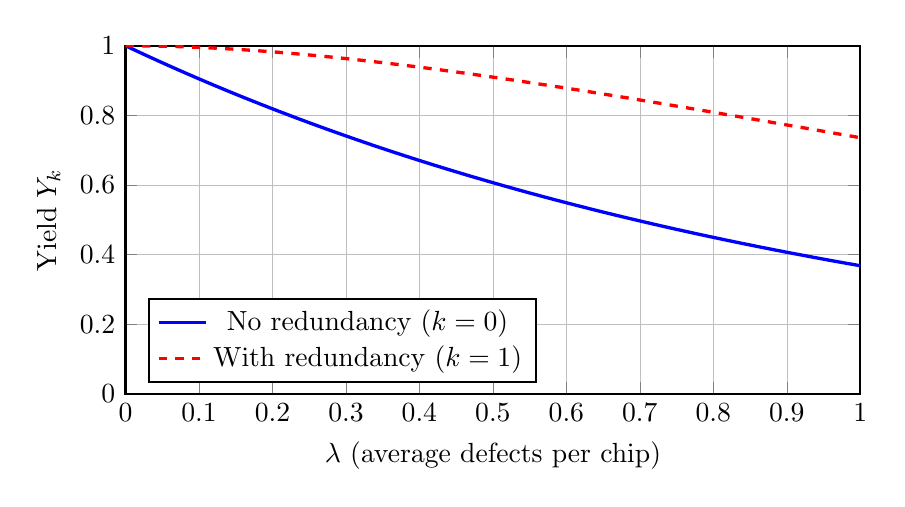
\begin{tikzpicture}
    \begin{axis}[
      width=0.9\linewidth,
      height=6cm,
      xlabel={$\lambda$ (average defects per chip)},
      ylabel={Yield $Y_k$},
      xmin=0, xmax=1,
      ymin=0, ymax=1,
      legend pos=south west,
      grid=both,
      major grid style={line width=.2pt,draw=gray!50},
      minor grid style={line width=.1pt,draw=gray!20},
      thick,
    ]
      % 冗長なし (k=0): Y0 = exp(-λ)
      \addplot[blue, very thick, domain=0:1, samples=200] {exp(-x)};
      \addlegendentry{No redundancy ($k=0$)}

      % 冗長あり (k=1): Y1 = exp(-λ) * (1+λ)
      \addplot[red, dashed, very thick, domain=0:1, samples=200] {exp(-x)*(1+x)};
      \addlegendentry{With redundancy ($k=1$)}
    \end{axis}
  \end{tikzpicture}
  \caption{Illustrative yield sensitivity (Poisson model) with and without redundancy.}
  \label{fig:yield}
\end{figure}

\section{Design Review Limitations}
Design reviews (DR) could only verify rule compliance and formal specifications.  
They failed to predict scalability risks arising from incomplete silicide phase transformation.  

Before this product generation, SRAM macros had already been integrated, but only up to the 500~kbit level, where the issue had not yet manifested.  
Based on those successful precedents, the team assumed that integration of a 1~Mbit macro would also be safe.  
However, the larger array size amplified single-bit failures, and the issue was not extracted during the initial development review stage.  

This case shows that DR without continuous empirical feedback was insufficient.

\section{Countermeasures}
\subsection{Provisional Measures}
Etch profiles were adjusted to slightly undercut sidewalls, ensuring sufficient separation between halo implants and active regions.  
This measure temporarily improved yield.

\subsection{Permanent Measures}
RTA conditions were optimized to stabilize C54 phase formation.  
However, this changed device parameters, requiring re-characterization of process-device models.

\section{Educational Application}
\subsection{Teaching Materials}
\begin{itemize}
    \item Cause-effect diagrams linking process $\rightarrow$ defect $\rightarrow$ yield
    \item Comparative tables: 0.25~µm vs 0.18~µm (technology vs HV integration)
    \item Exercises: process fix vs redundancy adoption
\end{itemize}

\subsection{Universality}
Trade-offs between technical stability and economic pressure remain relevant today.  
Similar cases exist in re-use of 28~nm FD-SOI or 40~nm BCD.

\section{Conclusion}
This historical case demonstrates that residual risks remain in legacy nodes.  
Yield degradation due to incomplete silicide phase transition highlighted the inseparability of process optimization and empirical feedback.  
The educational value lies in integrating such case studies into semiconductor engineering curricula.

\section*{References}
\begin{thebibliography}{99}
\bibitem{Sze2007} S. M. Sze and K. K. Ng, \textit{Physics of Semiconductor Devices}, 3rd ed. Hoboken, NJ: Wiley, 2007.
\bibitem{Wolf1986} S. Wolf and R. N. Tauber, \textit{Silicon Processing for the VLSI Era, Volume 1: Process Technology}. Sunset Beach, CA, USA: Lattice Press, 1986.
\bibitem{Colinge2004} J.-P. Colinge, \textit{Silicon-on-Insulator Technology: Materials to VLSI}, 3rd ed. Springer, 2004.
\bibitem{ITRS2001} International Technology Roadmap for Semiconductors (ITRS), ``Process Integration, Devices, and Structures,'' 2001.
\bibitem{Takeda1994} E. Takeda, C. Y. Yang, and A. S. Grove, ``Silicide technology for ULSI applications,'' \textit{IEEE Transactions on Electron Devices}, vol. 41, no. 12, pp. 2133--2141, Dec. 1994.
\bibitem{Chang1996} J. P. Chang and A. J. Steckl, ``Titanium silicide formation and stability in submicron CMOS technology,'' \textit{Journal of Applied Physics}, vol. 79, no. 9, pp. 4536--4364, 1996.
\end{thebibliography}

% ---------- Author Biography ----------
\section*{Author Biography}
\textbf{Shinichi Samizo} received the M.S. degree in Electrical and Electronic Engineering from Shinshu University, Japan.  
He worked at Seiko Epson Corporation on semiconductor memory and mixed-signal device development and contributed to inkjet MEMS actuators and PrecisionCore printhead technology.  
He is currently an independent semiconductor researcher focusing on process/device education, memory architecture, and AI system integration.\\
\emph{Contact:} \href{mailto:shin3t72@gmail.com}{shin3t72@gmail.com}\quad
\emph{GitHub:} \href{https://github.com/Samizo-AITL}{Samizo-AITL}.

\end{document}
